\documentclass[../thesis/thesis.tex]{subfiles}
\begin{document}
 \chapter{Results}

 \section{Classifier Experiment Set 1}

\begin{table}
\centering
\begin{tabular}{|l|r|r|r|}
\hline
\textbf{Classifier}  & \textbf{\% Correct} & \textbf{RMS Error} & \textbf{F-Measure} \\ \hline

\multicolumn{4}{|c|}{Nominal Balanced} \\ \hline
J48         						& 78.5                        & 0.277             & 0.784              \\ \hline
KStar       						& 74.4                        & 0.293             & 0.743              \\ \hline
\textit{Neural Network}      		& 71.9                        & 0.329             & 0.718              \\ \hline
\textit{K Nearest Neighbors}		& 68.8                        & 0.372             & 0.670              \\ \hline
Naive Bayes 						& 61.1                        & 0.358             & 0.605              \\ \hline
SMO         						& 58.0                        & 0.385             & 0.569              \\ \hline

\multicolumn{4}{|c|}{Nominal Unbalanced} \\ \hline
J48         						& 82.9                        & 0.288             & 0.824              \\ \hline
KStar       						& 82.6                        & 0.285             & 0.818              \\ \hline
\textit{Neural Network}      		& 78.5                        & 0.294             & 0.777              \\ \hline
Naive Bayes							& 66.2                        & 0.352             & 0.644              \\ \hline
\textit{K Nearest Neighbors}   		& 57.6                        & 0.425             & 0.563              \\ \hline
SMO         						& 57.5                        & 0.380             & 0.554              \\ \hline

\multicolumn{4}{|c|}{Numeric} \\ \hline
\textit{Linear Regression}     & 63.4                        & 0.659  &  -          \\ \hline
\textit{K Nearest Neighbors}   & 55.8                        & 1.195  &  -          \\ \hline
\textit{Neural Network} 	   & 50.2                        & 0.777  &  -          \\ \hline

\multicolumn{4}{|c|}{Thermosense \cite{beltran2013thermosense}} \\ \hline
K Nearest Neighbors	    & - & 0.346 & - \\ \hline
Neural Network			& - & 0.385 & - \\ \hline		
Linear Regression		& - & 0.409 & - \\ \hline
\end{tabular}
\caption{Classifier Experiment Set 1 Results}
\label{tab:results:set1}
\end{table}

Experimental results from the first set of experiments were overall excellent, results from them can be seen in \Fref{tab:results:set1}. In the unbalanced results, an accuracy of 82.9\% was observed, and in the balanced results, 78.5\%. 

\begin{figure}
\centering
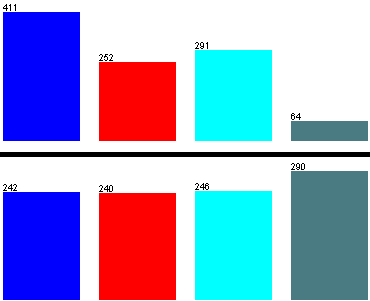
\includegraphics{../diagrams/temp/resample.png}
\caption{Experiment Set 1 Class Distribution Before and After Weka Re-sampling}
\label{fig:results:resample}
\end{figure}

Between the unbalanced and balanced classes, the ranking of different algorithms remained approximately the same, and consistently dropped in accuracy, with the exceptions being SMO, which increased in accuracy by 0.5\% in that instance, and, more notably, IBk, which increased in accuracy by 11.2\%. The drop in accuracy can be explained mostly by an over-representation of the zero class within the under-balanced data, as well as an underrepresentation of the three class (see \Fref{fig:results:resample}). These biases would enable classes to over-predict and under-predict these two classes respectively and achieve an artificially higher accuracy as a result. As discussed in the Methods, we performed re-sampling inside Weka to compensate for this.

For the numeric representation of the number of people, accuracy was consistently poor. In this instance, we calculate the ``correctly classified'' percentage by taking the predicted vs. actual results from Weka and rounding the predicted values to whole numbers, as a theoretical real-world solution may do to finalize its prediction. From this data, we can see that all three classifiers used performed consistently poorly, with the Root Mean Square Errors being consistently double or more of comparable nominal results. Interestingly, IBk was on-par with its nominal unbalanced partner, while the Multi-Layer Perceptron's accuracy dropped by more than 30\%.

The two highest accuracy classifiers, J48 and KStar, achieved quite similar results for both the balanced and unbalanced data while being quite different in implementation. % TODO: Why is this the case

\subsection{Individual sub-experiment results}

In addition to the above aggregate classification results, in which each of the nine sub-experiments results are combined and fed into the classifier, each of the sub-experiments has been individually classified with each of the six balanced nominal classifiers above. The results for these classifications can be seen in \Fref{tab:results:set1percent} and \Fref{tab:results:set1rmse}.



\begin{landscape}
\begin{table}
\centering
\begin{tabular}{|l|l|l|l|l|l|l|l|l|l|l|}
\hline
      & \textbf{1}     & \textbf{2}     & \textbf{3}     & \textbf{4}     & \textbf{5}     & \textbf{6}     & \textbf{7}     & \textbf{8}     & \textbf{9}     & \textbf{Avg}   \\ \hline
J48   & 86.0           & 88.4           & 72.7           & 65.4           & 72.8           & 90.9           & 76.9           & 80.7           & 80.2           & \textit{79.4}  \\ \hline
KStar & 86.0           & 91.7           & 76.9           & 65.4           & 72.8           & 91.7           & 82.3           & 82.6           & 80.2           & \textit{81.1}  \\ \hline
KNN   & 53.7           & 72.7           & 62.0           & 76.5           & 87.7           & 82.6           & 58.5           & 72.7           & 80.2           & \textit{71.9}  \\ \hline
Bayes & 84.3           & 59.5           & 75.2           & 65.4           & 72.8           & 87.6           & 75.4           & 77.6           & 67.9           & \textit{74.0}  \\ \hline
SMO   & 76.9           & 54.5           & 64.5           & 74.1           & 72.8           & 81.8           & 63.8           & 55.9           & 76.5           & \textit{69.0}  \\ \hline
ANN   & 84.3           & 83.5           & 86.0           & 75.3           & 88.9           & 85.1           & 73.1           & 77.0           & 92.6           & \textit{82.9}  \\ \hline
Avg   & \textit{78.5}  & \textit{75.1}  & \textit{72.9}  & \textit{70.4}  & \textit{78.0}  & \textit{86.6}  & \textit{71.7}  & \textit{74.4}  & \textit{79.6}  &                \\ \hline
\end{tabular}
\caption{Classifier Experiment Set 1 Individual Sub-experiment \% accuracy}
\label{tab:results:set1percent}
\end{table}

\begin{table}
\centering
\begin{tabular}{|l|l|l|l|l|l|l|l|l|l|l|}
\hline
      & \textbf{1}     & \textbf{2}     & \textbf{3}     & \textbf{4}     & \textbf{5}     & \textbf{6}     & \textbf{7}     & \textbf{8}     & \textbf{9}     & \textbf{Avg}   \\ \hline
J48   & 0.222          & 0.239          & 0.306          & 0.321          & 0.280          & 0.234          & 0.292          & 0.304          & 0.243          & \textit{0.271} \\ \hline
KStar & 0.189          & 0.209          & 0.280          & 0.317          & 0.272          & 0.208          & 0.277          & 0.267          & 0.243          & \textit{0.251} \\ \hline
KNN   & 0.439          & 0.347          & 0.427          & 0.284          & 0.245          & 0.281          & 0.415          & 0.333          & 0.290          & \textit{0.340} \\ \hline
Bayes & 0.267          & 0.357          & 0.301          & 0.320          & 0.284          & 0.264          & 0.336          & 0.322          & 0.297          & \textit{0.305} \\ \hline
SMO   & 0.321          & 0.379          & 0.375          & 0.349          & 0.327          & 0.345          & 0.388          & 0.372          & 0.357          & \textit{0.357} \\ \hline
ANN   & 0.193          & 0.240          & 0.251          & 0.295          & 0.209          & 0.235          & 0.316          & 0.272          & 0.178          & \textit{0.243} \\ \hline
Avg   & \textit{0.272} & \textit{0.295} & \textit{0.323} & \textit{0.314} & \textit{0.270} & \textit{0.261} & \textit{0.337} & \textit{0.312} & \textit{0.268} &                \\ \hline
\end{tabular}
\caption{Classifier Experiment Set 1 Individual Sub-experiment RMSEs}
\label{tab:results:set1rmse}
\end{table}
\end{landscape}

\section{Thermosense Comparison}

To aid in comparison with the Thermosense algorithm, in our experiment sets we chose three techniques similar to those used in Thermosense; an Artificial Neural Network (Multilayer Perceptron in Weka), K Nearest Neighbors (IBk in Weka) and Linear Regression. These techniques are highlighted in italics in the \Fref{tab:results:set1} ranking. We also use an experimental setup with 0--3 people, just as the Thermosense experiments do.

With this setup, we note that very similar balanced results were achieved for the Neural Network (0.329 ours vs. 0.385 theirs) and K Nearest Neighbors (0.372 ours vs. 0.346 theirs), while the numeric Linear Regression was significantly worse on ours (0.659 ours vs. 0.409 theirs).

With the Linear Regression model, the most striking difference to the Thermosense paper is evident, with a worsening of more than 46\% being shown. Looking more closely at the Linear Regression generated, \Fref{eq:linreg}, we can see that the impact of the three features on the model are minimal, with the algorithm choosing minuscule weights. This suggests that the algorithm was unable to find any strong correlation between the three features and the number of people.

\begin{equation} \label{eq:linreg}
n = 0.0783a + -0.0616b + -0.0331c + 0.4923
\end{equation}

However, none of the techniques used by Thermosense proved to be the best out of those algorithms tried. The Neural Network and K Nearest Neighbors techniques represent the middle-of-the-road of our results, with both being bested by the J48 and KStar algorithms, which produced RMSEs of 0.277 and 0.293 respectively. Both these results are significantly better than Thermosense's best RMSE of 0.346 for K Nearest Neighbors, with J48 representing a 28\% improvement over that technique.



 \ifcsdef{mainfile}{}{\bibliography{../references/primary}}
\end{document}
